\documentclass[a4paper, 12pt]{article}

\usepackage[utf8]{inputenc}
\usepackage[T1]{fontenc}
\usepackage{graphicx}
\usepackage[portuguese]{babel}
\usepackage[top=2cm,right=2cm,bottom=2cm,left=2cm]{geometry}
\usepackage{hyperref}
\usepackage{fontspec}
\setmainfont{Arial}

\begin{document}
	\begin{enumerate}
		\item[]\textbf{Questão 1} 
		
		\hspace{1cm}Tempo é o conjunto das condições atmosféricas de determinado lugar em determinado momento. Clima é a média das condições atmosféricas desse lugar; ou seja, é o resultado da repetição de um determinado tipo de tempo nesse lugar por anos sucessivos.
		
		\item[]\textbf{Questão 2} 
		
		\hspace{1cm}Representa os eventos que compõem o tempo atmosférico responsáveis pela caracterização do clima.
		
		\item[]\textbf{Questão 3} 
		
		\hspace{1cm}Fatores são agentes causais que
		condicionam os elementos meteorológicos, associados aos aspectos físicos.
		
		\href{http://www.leb.esalq.usp.br/leb/aulas/lce306/Aula2_2012.pdf}{Link}
		
		\item[]\textbf{Questão 4}
		
		\hspace{1cm}A radiação solar pode ser tomada
		tanto como elemento, por ser uma variável
		que quantifica a disponibilidade de energia
		solar na superfície terrestre, como também
		pode ser considerada um fator, por
		condicionar a temperatura, a pressão e
		indiretamente outros elementos meteorológicos
		
		\item[]\textbf{Questão 5} 
		
		\hspace{1cm}As estações do ano são estabelecidas com base na posição relativa Terra - Sol tomando-se o equador terrestre como referencial. Ao longo do tempo a Terra ao descrever um movimento de rotação e translação causa variação no ângulo de declinação solar ($\delta$). Ao descrever uma trajetória elíptica as regiões da Terra recebem diferentes níveis de luz incidente em sua superfície e isso torna o movimento aparente do Sol distinto ao longo do tempo. Dessa forma, é possível ter maior incidência de luz em um dos hemisférios, caracterizando os solstícios ou de forma igualmente distribuída na linha do Equador, o que caracteriza o equinócio. Logo, as diferentes taxas de energia absorvidas pelas diferentes regiões da Terra promovem a variação do gradiente de temperatura na sua superfície.
		
		\item[]\textbf{Questão 6} 
		
		\hspace{1cm}Os verões são caracterizados por elevadas temperaturas acompanhadas de altos índices pluviométricos. Nesse período, por estar no solstício de verão os dias são mais duradouros e a incidência solar aproxima-se da normal a superfície terrestre. No outono ocorre queda gradativa das temperaturas, exceto nas regiões próximas à linha do Equador. O inverno caracteriza-se pela queda das temperaturas, ocasionando ventos mais frios e secos, baixa umidade do ar, dias mais curtos e geadas em locais mais ao sul do país, podendo nevar em algumas partes. Na região Norte há maior ocorrência de chuvas no período. Por fim, a primavera é marcada pelo aumento gradativo das temperaturas antecedendo a chegada do verão. Juntamente a esse elemento, há elevação da umidade e ocorrência de chuvas.
		
		\item[]\textbf{Questão 7} 
		
		\hspace{1cm}Escalas espacial e temporal.
		
		\item[]\textbf{Questão 8}
		
		\hspace{1cm}A \textbf{macro-escala} trata dos fenômenos em escala regional ou geográfica. Caracteriza o macro-clima de grandes áreas em função dos fatores geográficos como: latitude, longitude, altitude, maritimidade, continentalidade e atuação de massas de ar. \textbf{meso-escala} associa-se aos eventos em locais, onde a topografia condiciona o topo-clima. As condições do relevo existente como exposição e configuração do terreno são responsáveis pela alteração dos fatores denominados ``topoclimáticos'', sendo estes de fundamental importância para o planejamento agrícola. A \textbf{micro-escala} é responsável por modificar as condições meteorológicas em uma pequena escala. Alguns fatores que modificam essas condições dizem respeito ao manejo utilizado no solo, retirada de cobertura vegetal, adensamento de plantio entre outras. Logo, diferentes sistemas de plantio como convencional e direto interferem de formas distintas o microclima local, por exemplo.
		
		\item[]\textbf{Questão 9} 
		
		\hspace{1cm}São associadas aos movimentos de translação e rotação da Terra, pois podem variar as condições temporais tanto num escala diária quanto anual.
		
		\item[]\textbf{Questão 10} 
		
		\hspace{1cm}Define-se variabilidade climática como uma variação das condições climáticas em torno da média climatológica. Com base nessa variação podem ser estabelecidos outros parâmetros como anomalias e mudanças climáticas.
		
		\begin{figure}[!h]
			\centering
			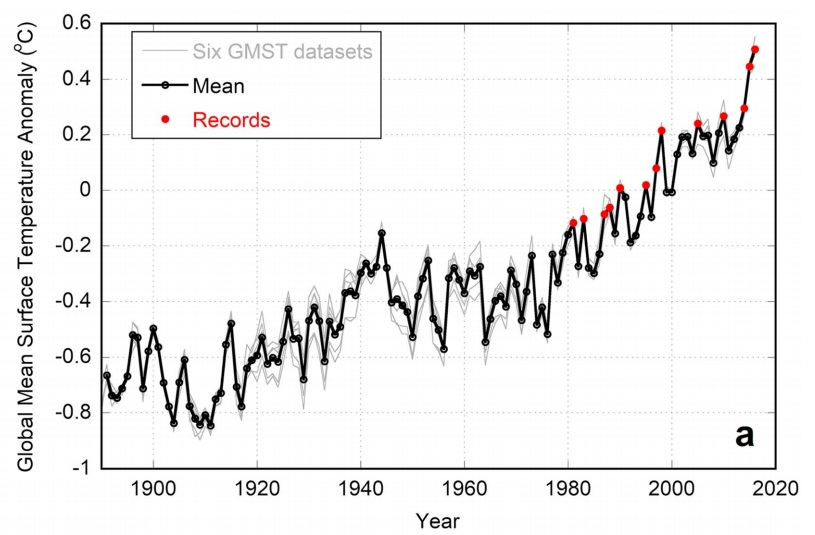
\includegraphics[scale=.65]{images/graphic.jpg}
			\caption{Gráfico representando o salto na temperatura global entre 1900 e 2020}
		\end{figure}
	\end{enumerate}
\end{document}